\documentclass[12pt]{article}

\usepackage{uw_rpt} 				% Template: Github.com/patrickkang/uwaterloo_wkrpt
\usepackage{graphicx} 				% Formatting of figures
%\usepackage{amsmath}				% Only used for Greek symbols
\usepackage{array}					% More options for tables
\usepackage{verbatim}				% I forget why this is required, but it is
\usepackage{minted} 				% For code snippets
\usepackage{finstrut}				% Scared to delete this one too
\usepackage{apacite} 				% Better APA format than the default
\usepackage{url} 					% Makes Github URLs look nice
\usepackage[section]{placeins} 		% Fixes placement of floats
\usepackage[labelfont=bf, font=small]{caption} 	% Makes "Figure x:" bold
%\usepackage{subfig}                 % For figures with a,b,c,etc.
\usepackage{titlesec}               % To reduce spacing between headers and text
\usepackage{longtable}
\usepackage{wrapfig}                % Wrap text around figures

% Fixes large amounts of whitespace around headers?
\titlespacing\section{0pt}{12pt plus 4pt minus 2pt}{0pt plus 1pt minus 1pt}
\titlespacing\subsection{0pt}{12pt plus 1pt minus 1pt}{0pt plus 1pt minus 1pt}

% Fixes Column sizes for tables
\newcolumntype{L}[1]{>{\raggedright\let\newline\\\arraybackslash\hspace{0pt}}m{#1}}
\newcolumntype{C}[1]{>{\centering\let\newline\\\arraybackslash\hspace{0pt}}m{#1}}
\newcolumntype{R}[1]{>{\raggedleft\let\newline\\\arraybackslash\hspace{0pt}}m{#1}}

% Fixes issue of the table being labelled as a figure
\def\table{\def\figurename{Table}\figure}
\let\endtable\endfigure 

\begin {document}

% \UWtitle{report title} { workplace } {Name and Date} %
\UWtitle{Inferring microRNA functions from genome-wide binding site occurrences}{
    Senior Honours Project (BIOL 499)\\
    Supervisor: Dr. Andrew Doxey\\
    2\textsuperscript{nd} Reader: Dr. Paul Craig
}{
	Mathias Renaud\\
	ID 20558745\\
	\today
}

% Acknowledgements %
\tocsection{Acknowledgements} 

I would like to thank Dr. Andrew Doxey for his support and guidance over the course of this project. Without his advice and encouragement, this project would not have been possible.

I also would like to thank Dr. Paul Craig for agreeing to be my second reader and helping determine the scope of the project.

Lastly, I would like to thank all members of the Doxey Lab. They helped me solve some technical problems and provided constructive feedback.

\newpage

% SUMMARY %
\tocsection{Summary} 
With diverse roles in essential biological processes such as differentiation, metabolic control, and metastasis, microRNAs (miRNAs) are key regulators of gene expression. These small, non-coding RNAs bind to specific target messenger RNAs as a mode of post-transcriptional repression. Differential expression of miRNAs has been shown to be an integral mechanism for specifying temporal- and tissue-specific gene expression patterns. While the effects of certain miRNAs on specific functions have been characterized, there are still many functional associations of miRNAs to be uncovered. Here we present the functional associations of over 120 miRNA families as predicted by a computational screen in \textit{Danio rerio} (zebrafish). Our computational pipeline uses genome-wide predicted targets of miRNA families to identify enriched functions under control of a given miRNA. To explore the validity of these bioinformatic predictions, select miRNAs were compared to experimental findings in the literature. Overall, this screen provides a foundation of many novel miRNA-function associations that can be characterized experimentally in future work.
\newpage

% TABLE OF CONTENTS %
\UWtableofcontents

% from here, page numbering is different. %
\pagenumbering{arabic}
\ifoot[]{}
\cfoot[]{}
\ofoot[\pagemark]{\pagemark}
\pagestyle{scrplain}


% Introduction %
\section{   Introduction}

\begin{wrapfigure}{R}{0.45\textwidth}
\centering
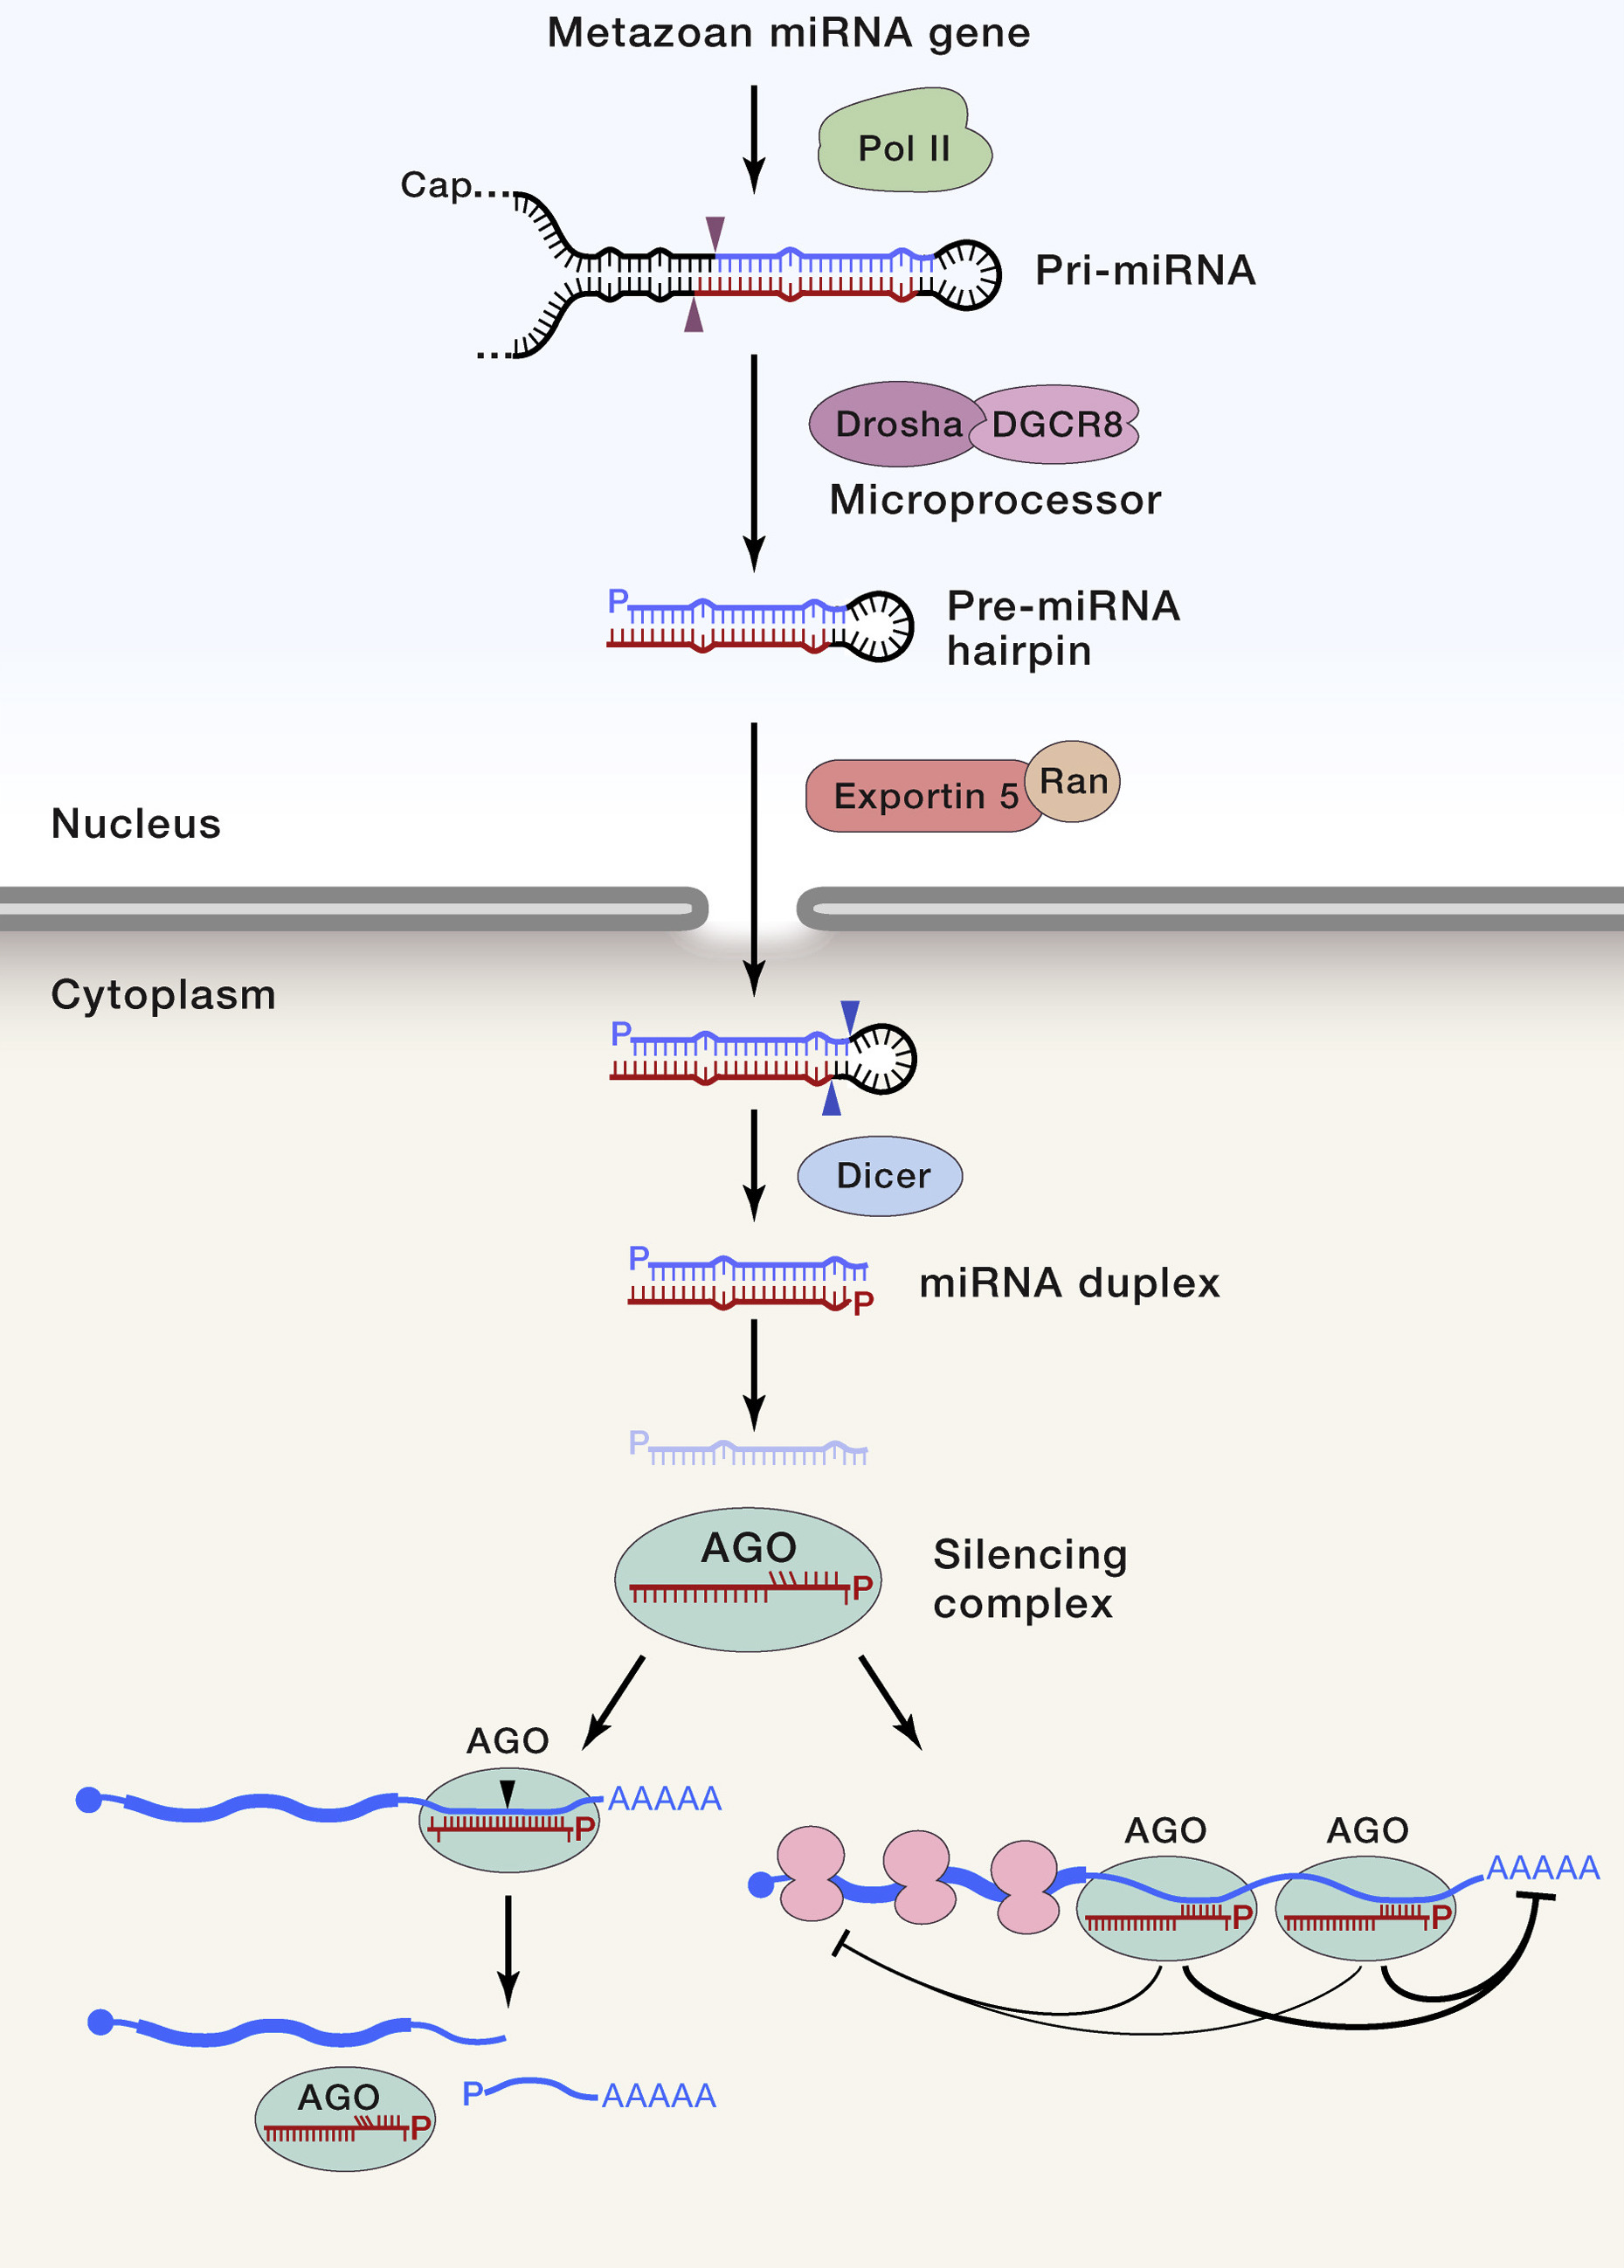
\includegraphics[width=0.45\textwidth]{figures/gr1_lrg.jpg}
\caption[microRNA Mechanisms]{Mechanism of microRNA biogenesis and regulation \cite{bartel2018metazoan}.}
\label{1}
\end{wrapfigure}

With diverse roles in essential biological processes such as differentiation, metabolic control, and metastasis, microRNAs (miRNAs) are key regulators of gene expression \cite{bartel2009micrornas, christopher2016microrna}. These small, non-coding RNAs (ncRNAs) specifically bind to target messenger RNAs (mRNAs) as a mode of post-transcriptional regulation. Mature miRNAs associate with argonaute proteins into a ribonucleoprotein complex called an RNA-induced silencing complex (RISC). The role of the miRNA in RISC is to recognize and bind to specific mRNA targets, leading to degradation or translational repression by the argonaute subunit, as shown in figure 1 \cite{filipowicz2008mechanisms, bartel2018metazoan}. Differential expression of miRNAs has been shown to be an integral mechanism for specifying temporal- and tissue-specific gene expression, as well as regulating oncogenes and initiating defences against viral or bacterial infection \cite{farh2005widespread, allison2012fundamental, andreassen2017mirnas}. MiRNAs are predicted to effect 30-60\% of protein-coding genes in mammals, and regulate nearly every cellular process \cite{andreassen2017mirnas, filipowicz2008mechanisms}. Therefore, it is not hard to imagine how dysregulation of miRNAs can contribute to a variety of different diseases.

In order to understand the effects of miRNAs on gene regulation, the interactions between miRNA and mRNA must be understood \cite{agarwal2015predicting}. The specificity of miRNA regulation comes from the binding to complementary ``target sites'' on mRNA transcripts, usually located in the 3$^\prime$ untranslated region (3$^\prime$UTR) \cite{bartel2009micrornas}. Through the development of early algorithms to predict miRNA-mRNA interactions, it was found that the minimal region necessary for successful binding was the ``seed'' region: positions 2-7 on the miRNA \cite{bartel2009micrornas}. Therefore target sites of a given miRNA can be classified based on their degree of complementarity to the corresponding miRNA’s seed, with each type differing in binding affinity \cite{bartel2009micrornas}. The unique sequence of a seed region is the attribute used to define miRNA families, with members of a family differing in positions outside of the seed but sharing a common set of targets \cite{bartel2009micrornas}. Target prediction algorithms, such as TargetScan, look for the reverse complement of the seed region of a miRNA within a set of test regions, while taking into account the different types of target sites that can occur \cite{lewis2005conserved}. The resulting locations of target sites can predict which genes may be under the control of a given miRNA.

To understand the major roles that specific miRNA families play in the regulation of biological processes, it is necessary to translate sets of target sites into functional annotations. This can be done by determining a set of functional annotations that are significantly enriched in the predicted targets of a miRNA family, compared to the full set of genomic regions from which the targets were predicted. One method to do this is Genomic Regions Enrichment Analysis Tool (GREAT). GREAT is a functional enrichment method that uses a genomic region-based approach, rather than the gene-based approach that other tools employ, to more accurately model genomic regulatory regions \cite{hiller2013computational}. Additionally, while other methods exclusively use gene ontology (GO) terms, GREAT includes many more ontologies for human, mouse, and zebrafish genomes. This allows for connections to be made between the different ontologies to identify common functions that are more likely to be biologically accurate.

% Figure 2 %
\begin{figure}[]
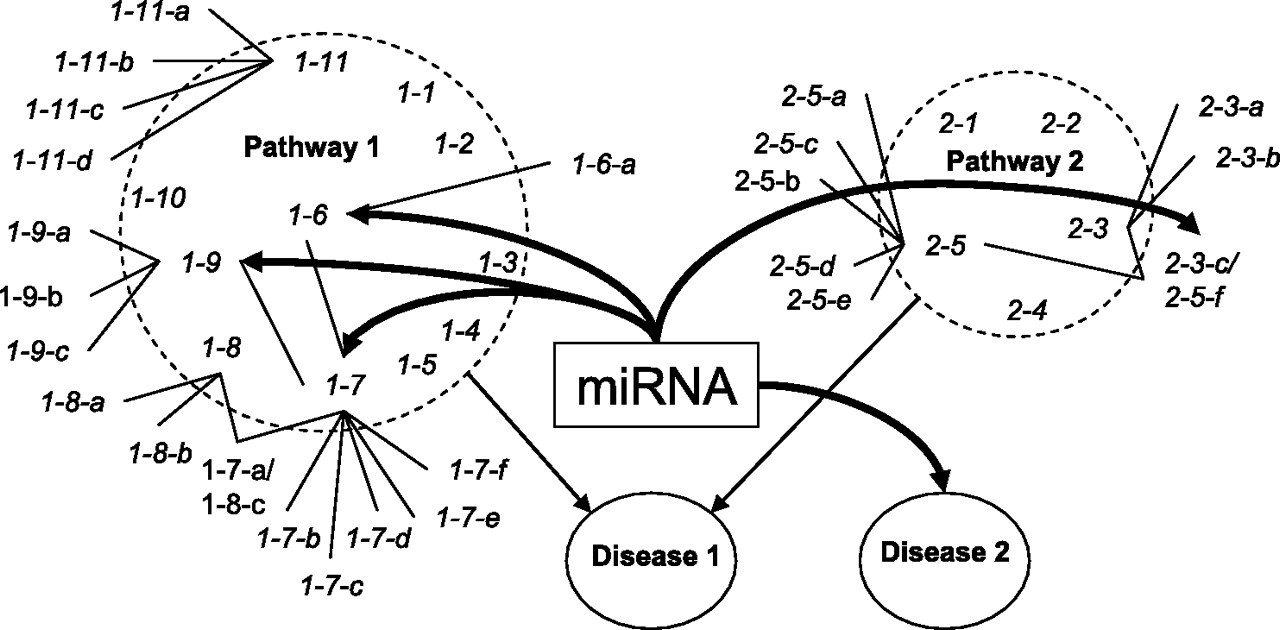
\includegraphics[width=.5\textwidth]{figures/zh70100933700002.jpeg}
\centering
\caption[Consequences of microRNA Dysregulation]{The many consequences of microRNA dysregulation. This hypothetical regulatory network diagram shows how a single microRNA family can regulate many different pathways and multiple members of these pathways. The result is that dysregulation in a single microRNA family can have  cascading effects, leading to various disease phenotypes \cite{liang2009microrna}.}
\centering
\label{2}
\end{figure}

One reason why it is so important to understand miRNA function is that dysregulation of miRNAs is often implicated in a wide range of diseases, especially cancers \cite{lu2008analysis, gebeshuber2013mir}. Figure 2 demonstrates how dysregulation of a single miRNA family can have widespread effects on many members of multiple pathways \cite{liang2009microrna}. Presently, most studies on miRNA function characterize the effect of a single miRNA on a specific function, but there are still an abundance of miRNA functions yet to be uncovered. Therefore, the purpose of the project was to develop a method that can predict the functions of all miRNA families in an organism. Once developed, this method was applied to perform a genome-wide computational screen in \textit{Danio rerio} (zebrafish) to explore predicted functional associations of miRNAs.

% Methods %
\section{   Methods}

\begin{wrapfigure}{R}{0.45\textwidth}
\centering
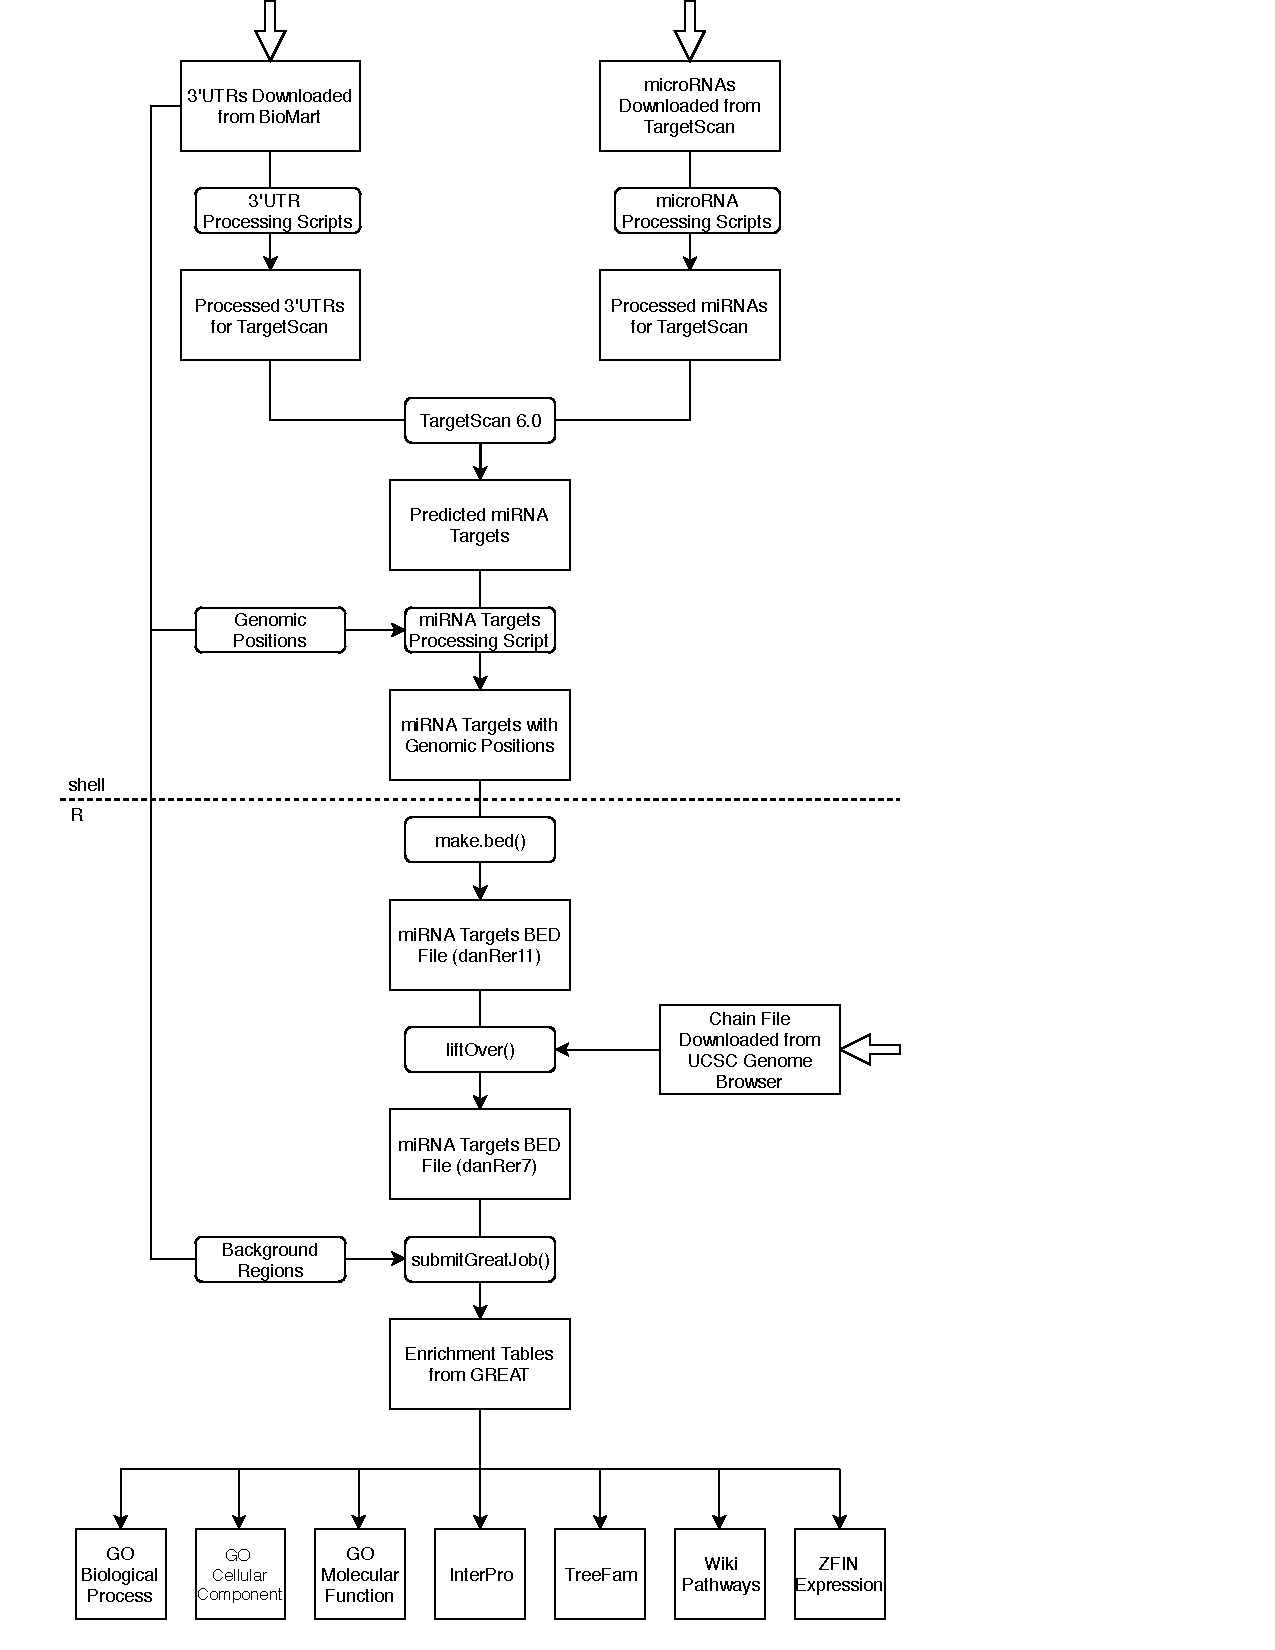
\includegraphics[width=0.45\textwidth]{figures/pipeline.pdf}
\caption[Computational Pipeline]{Flow chart depicting the steps of the computational pipeline developed to predict functional associations of microRNAs.}
\label{1}
\end{wrapfigure}
The computational pipeline used to generate the data for this screen was made up of existing methods for miRNA target prediction and functional annotation, as well as bespoke scripts to clean the input data, link the various tools, and generate output tables and figures (Figure 3). TargetScan 6.0 was first used to predict the target sites of miRNAs \cite{lewis2005conserved}. Since the precomputed predictions from TargetScanFish were outdated by multiple genome assemblies, it was decided to run the algorithm locally on the most recent zebrafish assembly. The sequences of all 215 miRNA families in zebrafish were downloaded from TargetScanFish 6.2. After collapsing families with identical seed regions (e.g. miR-29a and miR-29b), the input consisted of 126 unique miRNA families. The target sites for these miRNA families were searched for in all known 3’$^\prime$UTRs in zebrafish, which were downloaded from BioMart (Ensembl v95) and included the genomic positions of the sequences \cite{zerbino2017ensembl}. This initial screen was restricted to 3’$^\prime$UTRs since most miRNA-directed silencing occurs due to binding within this region \cite{bartel2009micrornas}.

The 3’$^\prime$UTR input file required extensive processing before targets could be predicted. This included removing 3’$^\prime$UTRs that mapped to extrachromosomal scaffolds and those with no sequence available. 15,810 3’$^\prime$UTRs in the set had duplicate identifiers due to different isoforms of a transcript having different length 3’$^\prime$UTRs. For these cases, only the longest 3$^\prime$UTR for each duplicate ID was kept to prevent overrepresentation of targets on genes that have multiple isoforms (keep-longest.py: \url{gist.github.com/mkweskin/8869358}). Another complexity of this dataset was 3’$^\prime$UTRs spanning multiple exons, of which there were 2,108 entries that had multiple sets of indices defining the boundaries of the many exons. These 3’$^\prime$UTRs were split into separate entries for each exon so that genomic position calculations could be done for targets in those UTRs. After preprocessing, there were 22,659 unique 3’$^\prime$UTRs to be scanned for miRNA target sites.

For each predicted target, TargetScan provided the corresponding gene identifier, the type of target site, and the position of the target site within the UTR. The position of the target site within the UTR sequence together with the genomic position of each UTR was used to determine the genomic position of each target site. The resulting genomic positions of target sites for each miRNA family were converted into BED format to be sent to the GREAT web server using the ‘rGREAT’ package \cite{gu2018}. First, the target sites predicted for the GRCz11/danRer11 (May 2017) zebrafish assembly had to be converted to the Zv9/danRer7 (July 2010) assembly used by GREAT, using the LiftOver algorithm and chain file from UCSC genome browser \cite{karolchik2003ucsc}. GREAT was used to determine the set of annotation terms that were significantly enriched in the targeted regions for each miRNA compared to the background of all tested 3’$^\prime$UTRs for seven ontologies using a foreground/background hypergeometric test (Table 1). The foreground set of predicted miRNA target sites was tested against a background set consisting of the 3’$^\prime$UTRs that were used to predict the sites, as a whole genome background was not appropriate for this analysis \cite{rhee2008use}. The output retrieved from GREAT was all significantly enriched (Bonferroni-corrected p-value $<$ 0.05) terms for each of the seven ontologies. All code and data used in this analysis is available at \url{github.com/MathiasRenaud/BIOL499}.

% Results %
\section{   Results}

This study provides an up-to-date genome-wide screen for 3’$^\prime$UTR miRNA targets in zebrafish for the 126 known miRNA families. A total of 438,606 unique target sites were predicted. There was an average of 3,481 targets per miRNA family, ranging from 257 targets for miR-126a to 21,215 targets for miR-740. To derive biological meaning from the large number of targets, functional enrichment analysis was performed on the full set of predicted targets for each miRNA family. Table 1 summarizes the number of significantly enriched miRNA-function associations for each of the seven ontologies provided by GREAT for zebrafish. A total of 288,816 significantly enriched terms (p $<$ 0.05) were detected across all miRNA families after Bonferroni correction.
%-----------------------------------------------------------------------------
% Table 1 %
\begin{table}[h!]
\centering
\captionof{table}[Summary of Ontologies]{Summary of the ontologies provided for zebrafish by GREAT
}
\resizebox{\textwidth}{!}{
\begin{tabular}{lrrl}
\textbf{Ontology}               & \textbf{Total Number of Terms} & \textbf{Number of Significant Associations} & \textbf{Citation} \\\hline
GO Biological Function & 4067                  & 46950                              & Ashburner et al., 2000 \\
GO Cellular Component  & 640                   & 5134                               & \\
GO Molecular Function  & 1807                  & 13257                              & \\
WikiPathway            & 8034                  & 38794                              & Pico et al., 2008 \\
InterPro               & 6396                  & 22576                              & Hunter et al., 2009 \\
TreeFam                & 105                   & 2111                               & Ruan et al., 2008 \\
WT Expression          & 11422                 & 159994                             & Howe et al., 2013 \\\hline
\textbf{Total}                  & \textbf{32471}                 & \textbf{288816}                             & 
\end{tabular}
}
\\
\begin{flushleft}{\scriptsize Table 1 shows the number of unique terms for each of the seven ontologies used in this study and the number of significantly enriched (p $<$ 0.05) associations predicted across the 126 microRNA families.}\end{flushleft}
\label{1}
\end{table}
%-----------------------------------------------------------------------------

For each miRNA family tested, an enrichment table for each of the seven ontologies was generated. These included the identifier and name of each term, as well as all relevant statistics from the foreground/background hypergeometric test over genomic regions. As an example of the output, table 2 below shows the top three GO biological function hits for miR-29a (transposed to fit page). The different fields describe the total number genomic regions associated with the term, how many hits are expected by chance, the observed number of hits, and the resulting fold enrichment and statistical significance for that term in the provided foreground set compared to the background. The terms in each table are ranked by statistical significance. In this example you can see how the data within these tables can elucidate the functions regulated by a miRNA family; in this case metabolism of nucleotides is predicted to be one of the main processes under the control of miRNA-29a.

%-----------------------------------------------------------------------------
% Table 2 %
\begin{table}[h!]
\centering
\captionof{table}[Example Output]{Example output enrichment table}
\resizebox{\textwidth}{!}{
\begin{tabular}{lrrr}
\hline
\textbf{ID}                          & GO:0046113                   & GO:0006206                              & GO:0006208                              \\
\textbf{name}                        & nucleobase catabolic process & pyrimidine nucleobase metabolic process & pyrimidine nucleobase catabolic process \\
\textbf{Total Regions}               & 27                           & 26                                      & 22                                      \\
\textbf{Expected Regions}            & 2.145                        & 2.065556                                & 1.747778                                \\
\textbf{Foreground Region Hits}      & 12                           & 10                                      & 9                                       \\
\textbf{Fold Enrichment}             & 5.594406                     & 4.841313                                & 5.149396                                \\
\textbf{Region Set Coverage}         & 0.005994006                  & 0.004995005                             & 0.004495504                             \\
\textbf{Term Region Coverage}        & 0.4444444                    & 0.3846154                               & 0.4090909                               \\
\textbf{Foreground Gene Hits}        & 4                            & 4                                       & 3                                       \\
\textbf{Background Gene Hits}        & 6                            & 8                                       & 5                                       \\
\textbf{Total Genes Annotated}       & 9                            & 11                                      & 8                                       \\
\textbf{Raw p-value}                 & 3.44E-07                     & 1.59E-05                                & 2.37E-05                                \\
\textbf{Bonferroni-adjusted p-value} & 0.001                        & 0.029                                   & 0.029   \\\hline                                 
\end{tabular}
}
\\
\begin{flushleft}{\scriptsize Table 2 shows all fields that are provided for each ontology table. The example data is the top three hits in the GO Biological Process ontology for miR-29a.}\end{flushleft}
\label{1}
\end{table}
%-----------------------------------------------------------------------------

To determine the strongest miRNA-function associations, the enriched terms for each ontology were pooled and ranked by Bonferroni-corrected p-value. Table 3 lists the top five terms from the ranked list for each ontology. These highly enriched functions suggest specialized regulatory roles of certain miRNA families, as well as processes that are dependent on miRNA control.

%-----------------------------------------------------------------------------
% Table 3 %
\begin{table}[h!]
\centering
\captionof{table}[Top Ranked Annotations]{Top ranked terms based on enrichment across all miRNA families}
\resizebox{\textwidth}{!}{
\begin{tabular}{llll}
\textbf{Ontology}          & \textbf{Term}                                                    & \textbf{Adjusted p-value} & \textbf{miRNA Family}           \\\hline
GO Biological Process & intra-Golgi vesicle-mediated transport                  & 3.06E-39         & dre-miR-184            \\
                      & apoptotic process/programmed cell death                 & 4.78E-32         & dre-miR-199            \\
                      & cell death                                              & 7.93E-29         & dre-miR-199            \\
                      & Golgi vesicle transport                                 & 6.38E-27         & dre-miR-184            \\
                      & lifelong otolith mineralization                         & 8.07E-25         & dre-miR-2191           \\\hline
GO Cellular Component & Golgi transport complex                                 & 1.34E-42         & dre-miR-184            \\
                      & protein serine/threonine phosphatase complex            & 3.78E-40         & dre-miR-18a/b/c        \\
                      & anaphase-promoting complex                              & 2.72E-17         & dre-miR-17a/20a/20b/93 \\
                      & apical junction complex                                 & 3.12E-13         & dre-miR-2191           \\
                      & tight junction                                          & 3.19E-13         & dre-miR-2191           \\\hline
GO Molecular Function & cysteine-type endopeptidase activity                    & 5.86E-45         & dre-miR-199            \\
                      & protein phosphatase type 2A regulator activity          & 5.79E-39         & dre-miR-18a/b/c        \\
                      & cysteine-type peptidase activity                        & 1.35E-38         & dre-miR-199            \\
                      & phosphatase regulator activity                          & 1.82E-33         & dre-miR-18a/b/c        \\
                      & cysteine-type endopeptidase activity                    & 4.61E-23         & dre-miR-204            \\\hline
Wiki Pathways         & Glycogen Metabolism                                     & 5.23E-35         & dre-miR-18a/b/c        \\
                      & Wnt Signaling Pathway                                   & 1.79E-25         & dre-miR-18a/b/c        \\
                      & IL-6 Signaling Pathway                                  & 1.88E-23         & dre-miR-18a/b/c        \\
                      & Wnt Signaling Pathway and Pluripotency                  & 3.70E-23         & dre-miR-18a/b/c        \\
                      & ErbB signaling pathway                                  & 1.67E-16         & dre-miR-726            \\\hline
InterPro              & Transmembrane protein 43 family                         & 8.16E-84         & dre-miR-730            \\
                      & Caspase-7                                               & 9.67E-76         & dre-miR-199            \\
                      & Peptidase C14                                           & 6.04E-58         & dre-miR-199            \\
                      & Transmembrane protein 43 family                         & 1.52E-55         & dre-miR-2191           \\
                      & Peptidase C14, caspase domain                           & 1.77E-55         & dre-miR-199            \\\hline
TreeFam               & wu:fi09b08, zgc:173770, zgc:173837                      & 6.67E-56         & dre-miR-138            \\
                      & cog6                                                    & 7.55E-44         & dre-miR-184            \\
                      & g3bp1, g3bp2, zgc:56304                                 & 2.46E-39         & dre-miR-138            \\
                      & asb7                                                    & 1.05E-29         & dre-miR-184            \\
                      & fam210a, si:ch211-105d11.2, zgc:112435                  & 3.32E-29         & dre-miR-2197           \\\hline
ZFIN WT Expression    & Segmentation:10-13 somites 14-16h; trigeminal placode   & 2.19E-22         & dre-miR-2193           \\
                      & Pharyngula:Prim-5 24-30h; statoacoustic (VIII) ganglion & 1.03E-20         & dre-miR-2193           \\
                      & Hatching:Long-pec 48-60h; amacrine cell                 & 1.78E-19         & dre-miR-733            \\
                      & Segmentation:26+ somites 22-24h; neural crest cell      & 4.35E-19         & dre-miR-733            \\
                      & Hatching:Long-pec 48-60h; corpuscles of Stannius        & 4.02E-17         & dre-miR-733m \\\hline
\end{tabular}
}

\begin{flushleft}{\scriptsize Table 3 shows the top five overall terms for each ontology across all miRNA families, based on Bonferroni-corrected p-value. This representation of the enriched annotations allows for easy identification of the strongest associations.}\end{flushleft}
\label{1}
\end{table}
%-----------------------------------------------------------------------------
To comprehend the large number of enriched terms and uncover more about the interrelated roles of various miRNA families, a heatmap was generated for each ontology. These figures display both clusters of miRNA families that regulate the same function and clusters of functions that are regulated by the same miRNA family. Figure 4 is the heatmap for the WikiPathways ontology (see \url{github.com/MathiasRenaud/BIOL499/Appendix} for the other 6 ontologies).
%-----------------------------------------------------------------------------
% Figure 4 %
\begin{figure}[]
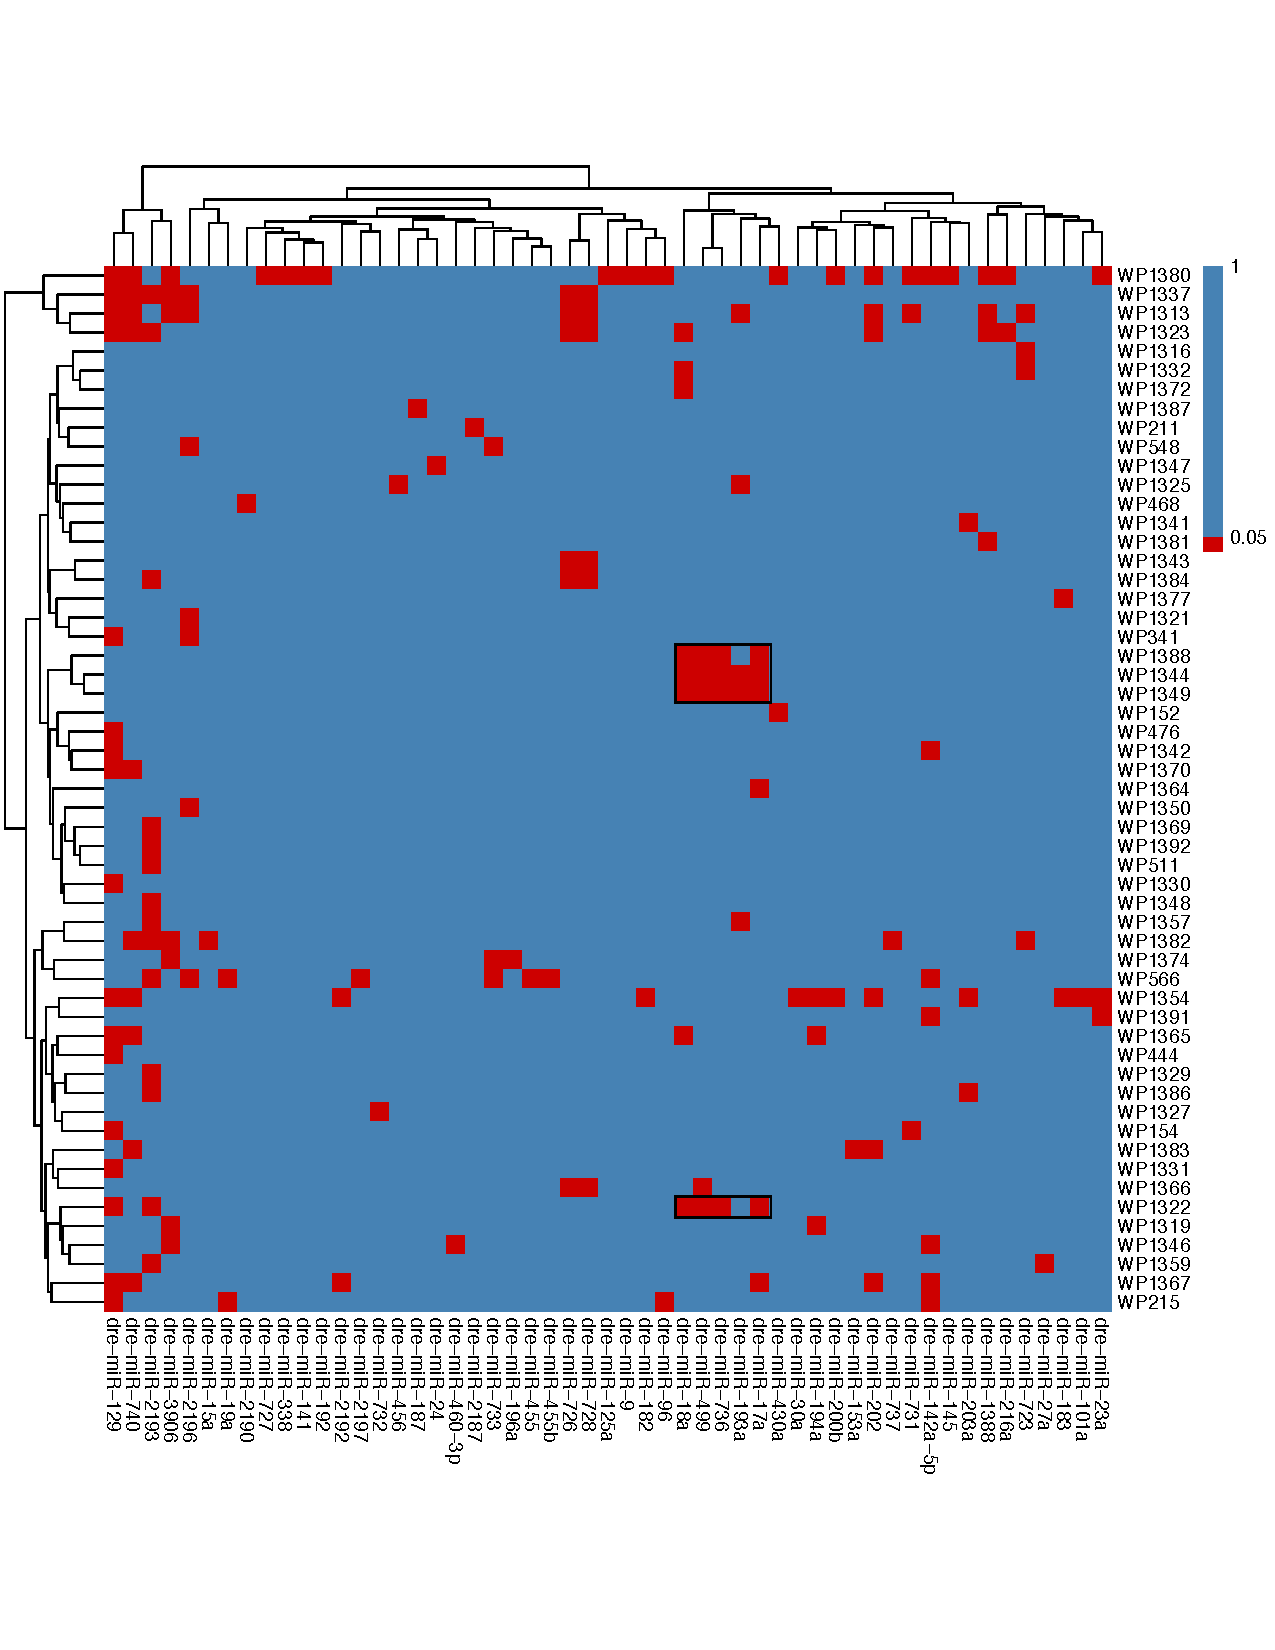
\includegraphics[width=\textwidth]{figures/heatmap.pdf}
\caption[WikiPathways Heatmap]{WikiPathways heatmap. The miRNA families with at least one significant association are along the x-axis while ontology terms with at least one significant association are along the y-axis. Red cells represent significantly enriched associations (Bonferroni-corrected p-value $<$ 0.05). Black boxes highlight areas mentioned in the discussion.}
\centering
\label{4}
\end{figure}
%-----------------------------------------------------------------------------


% Discussion %
\section{   Discussion}
The data presented in this computational screen of zebrafish miRNA targets provides a more comprehensive view of the functions regulated by individual miRNA families. Many studies have implicated an individual miRNA family in the regulation of a specific process. For example, a 2008 study by Woltering and Durston reported that miR-10 represses HoxB1a and HoxB3a. Although studies such as these are important for understanding the effects of miRNAs on specific processes, it suggests that the main role of miR-10 is to regulate HoxB genes. From this screen, the hox gene family was in fact significantly enriched for miR-10 (adj-p = 0.02) but blvra (biliverdin reductase A) was also enriched (adj-p = 0.001). Additionally, all significant terms across the other ontologies were biliverdin reductase functions (heme catabolic process, porphyrin-containing compound catabolic process, biliverdin reductase activity; adj-p $<$ 0.05). This suggests that the main function of this miRNA family may be heme metabolism, while regulation of Hox genes is a secondary role. Without considering functions associated with all predicted targets for a miRNA family, this potentially more prominent role of miR-10 would not have been known as no studies to date have looked at miRNA control of biliverdin reductase expression.

This example also shows how predicting all functions of miRNAs can uncover novel, uncharacterized regulatory roles and provide a better understanding of how certain processes are controlled. This is especially true of miRNAs which were predicted to have strong functional associations but have not yet been studied in zebrafish. An example of this is miR-184, which topped many of the ranked ontology term lists with highly significant associations, including three of the top ten GO Biological Process and TreeFam terms, as well as the top GO Cellular Component term (see Table 3). These highly enriched functions were concordant for golgi transport-associated terms including vesicle-mediated intracellular transport, protein ubiquitination/modification, and exocytosis. Additionally, all significantly associated expression patterns were those of the developing nervous system (brain nuclei and neural tube at 19-30h post-fertilization). Together, these predictions propose an important role in regulating the trafficking of neuronal signals in the developing zebrafish. MiR-184 regulates a relatively small set of targets (682 predicted), which supports the idea that it is specialized to regulate this specific function. Although the role of this miRNA has not been explored experimentally in zebrafish, studies in mice have shown that it is involved in proliferation and differentiation of neural stem cells, as well as cytokine release by microglia \cite{liu2010epigenetic, danis2016differential}.

In addition to predicting novel functions of miRNAs, the data resulting from this method also supports known biology. A 2013 study showed that over-expression of miR-100 inhibited tumour growth in breast cancer cell culture by down-regulating insulin-like growth factor 2 (IGF2) \cite{gebeshuber2013mir}. In this study, the top two GO Biological Process terms for miR-100 were regulation of cell proliferation (p $<$ 0.01). Additionally, the GO Molecular Function ontology for this miRNA included IGF1 and IGF2 binding in the top hits (p $<$ 0.01). This paper is just one among many that has linked this miRNA to development of cancer ($>$80\% of instances of ``miR-100'' on Google Scholar), which provides further confidence in the prediction of miR-100 being a regulator of cell proliferation.

The heatmaps for the individual ontologies highlight groups of miRNAs that may co-regulate the same function and groups of functions that may be regulated by the same miRNA. Visualizing these patterns allows for the identification of overlapping or co-operative control by miRNA families. In the WikiPathways heatmap in figure 4, the black boxes identify a group of four miRNA families (miR-17a, miR-18a, miR-499, and miR-736) that are all predicted to regulate the same four pathways (Wnt signalling, Wnt signalling and pluripotency, IL-6 signalling, and glycogen metabolism). As an additional example of predicting known biology, all of these miRNAs have previously been shown to regulate at least one of these pathways in other species \cite{andreassen2013discovery, brock2011microrna, wilson2010dynamic}. Without them being studied in zebrafish, this method was able to predict functions of these miRNAs that have been shown experimentally in other organisms.

\subsection{Conclusions}

To summarize, a computational pipeline was developed to predict the functions that are significantly associated with miRNA families to better understand the specific biological roles of miRNAs. This pipeline was applied to miRNA families in zebrafish to produce a vast quantity of significantly enriched functional annotation terms. The exploration of these select miRNAs highlight the wealth of knowledge provided by this method and demonstrate how the data within this initial screen could be the basis for future scientific inquiry.

\subsection{Future Directions}

The next steps for this project include improvements to the computational pipeline and testing of predictions in vivo. By implementing weighting of target sites by context score, the predictions can be improved. The context score of a target site determines the relative likelihood of binding by taking into account many factors such as evolutionary conservation, position of the site within the UTR, AU content, presence of secondary structures, and seed pairing stability \cite{agarwal2015predicting}. Addition of this feature will allow for ranking of target sites that will improve the biological accuracy and quality of the predictions. The predictions likely to be tested experimentally include the regulation of glycogen metabolism by miR-18 and regulation of fin morphogenesis by miR-2196.

\newpage
% References %
\bibliographystyle{apacite}
\bibliography{499.bib}
\newpage

% Appendix A %
%\tocsection{Appendix}
%\newpage

\end{document}